% !TeX spellcheck = en_GB

\documentclass{IEEEcsmag}

\usepackage[colorlinks,urlcolor=blue,linkcolor=blue,citecolor=blue]{hyperref}

\usepackage{upmath}
\usepackage{tikz}
\usepackage{graphicx}
\usepackage{subfigure}
\usetikzlibrary{arrows, positioning, automata}

% Flowchart
\tikzstyle{process} = [rectangle,
	minimum width=2cm, 
	minimum height=1cm,
	text centered, 
	draw=black, 
]
\tikzstyle{zk} = [rectangle,
	rounded corners=15pt,
	minimum width=2cm, 
	minimum height=1cm,
	text centered, 
	draw=black, 
	%fill=red!30
]	
\tikzstyle{startstop} = [rectangle, minimum width=3cm, minimum height=1cm, text centered, draw=black]
\tikzstyle{arrow} =[thick,->,>=stealth]


\jvol{XX}
\jnum{XX}
\paper{8}
\jmonth{May/June}
\jname{IT Professional}
\pubyear{2019}
\newtheorem{theorem}{Theorem}
\newtheorem{lemma}{Lemma}

\setcounter{secnumdepth}{0}

\begin{document}

\sptitle{Department: Head}
\editor{Editor: Name, xxxx@email}

\title{Easily Building Privacy-enabled Blockchain Applications}

\author{Marta Bell\'es-Mu\~noz}
\affil{iden3, Universitat Pompeu Fabra}

\author{Jordi Baylina}
\affil{iden3}

\author{Vanesa Daza}
\affil{Universitat Pompeu Fabra}

\author{Jos\'e L. Mu\~noz}
\affil{Universitat Politècnica de Catalunya}

\markboth{Department Head}{Paper title}

\begin{abstract}
For many enterprises and individuals the inability to conduct secure 
private transactions has been a major obstacle to 
fully embracing public blockchain networks. 
In this paper, we provide an overview of how zero-knowledge proofs (ZKPs)
allow getting both transparency and privacy in public ledgers.
With a use case, we describe how to build a privacy-enabled 
blockchain application using ZKP and present the software tools 
we have developed to facilitate the process to high level practitioners. 
\end{abstract} 


\maketitle
\chapterinitial{Public} ledgers are a disruptive tool for enabling interaction
between parties that do not have previous trust.
If the ledger state is considered a universal source of truth,
trust can be based on the certainty that interactions 
will be performed exactly as defined in the ledger.
This idea contrasts with the traditional approach, in which business relationships are 
based on legal contracts and reputation gained with previous interactions. 

Blockchain is the main technology to build 
public ledgers in a distributed way.
Essentially, blockchains work using a
distributed consensus algorithm that allows 
the network participants to deterministically update the
ledger state.
Ledger state changes are performed by transactions and in public distributed ledgers, 
each transaction is public (transparent) and 
remains immutable once ordered by the consensus algorithm. 

Many public ledgers also provide the capability of using smart contracts, which are pieces of code that define a set of
functions that implement business logic.
Smart contracts, as everything, are deployed in the ledger through a transaction. 
Once a smart contract is deployed, 
it is possible to modify the ledger 
state by sending a transaction calling a smart contract function that will make 
the changes according to its predefined logic.


The high transparency of traditional public ledgers is a desirable feature but
it is a concern when dealing with privacy,
understood as the right of each individual or legal entity to control the degree 
to which their personal or business information is shared with the environment.
To this respect, the interest of society and regulators about data confidentiality  
and privacy has grown in the recent years for both individual's privacy and industry trade secrets. 

For example, the need to guarantee 
individuals' privacy has ended with new 
legislation like the General Data Protection Regulation (GDPR) of the European Union. 
In the case of blockchain and industry, 
permissioned ledgers, which require an access control layer, appeared as a solution to enterprises and individuals that needed better privacy. 
However, security of blockchains rely on having a large number of participants contributing to the system. Hence, 
privacy and confidentiality should to be addressed by other means 
rather than by restricting participation. 

Although transparency and privacy may seem contradictory terms, it is possible to have both using a set of cryptographic tools called Zero-Knowledge Proofs (ZKP). 
ZKPs currently play an important role in the adoption of 
enterprise-friendly blockchain applications over public blockchains.

In the rest of the paper, we will provide an overview of ZKPs,
we will describe how to build a privacy-enabled blockchain application with
a use case and we will present our software implementations to make
this process easier to developers and researchers.


\section{ZKPs AND BLOCKCHAIN}

Zero-knowledge Proofs (ZKPs) are cryptographic protocols that 
enable one party, called prover, to convince another, called 
verifier, that a statement is true without revealing any 
information beyond the veracity of the statement. 
In plain words, these protocols allow you to prove that you know a secret 
without leaking any information about it.

ZKPs were revolutionary because for the first time in 
cryptography, instead of looking for secure communications 
in which some of the parties are trusted, the goal was to
establish trust between distrustful parties. 
The first generation of these protocols worked the following way: 
the verifier sent some challenges to the 
prover to check that, in fact, he knew the secret 
information, but the answers from the prover did not allow 
the verifier to reconstruct any part of the secret. 
Hence, ZKPs not only protect verifiers 
against malicious provers but also provers from malicious 
verifiers that want to obtain information from the prover.

One of the variants of these protocols 
are the so-called Non-Interactive ZKPs (NIZK), in which the prover 
can generate all the proof himself without need to interact 
with the verifier. 
NIZKs are very suitable for blockchain applications because the prover 
can create the proof and send it as part of a transaction to a smart contract.
Then, the smart contract can act as verifier and perform some 
action depending on whether the proof is valid or not.
Among NIZK protocols, the most interesting ones for blockchain are those ones
whose proof size is small and verification time is also short. 


This type of NIZK protocols that have succinct proof size 
and constant verification time exist and are called zk-SNARKs \cite{pinnochio}.  
This two properties led to achieve the duality privacy and transparency
with a huge impact in public distributed ledgers.
A prominent practical example is Zcash \cite{zcash}, a blockchain based on bitcoin,
that uses zk-SNARKs in its core protocol for verifying that private 
transactions (named ``shielded" transactions) have been correctly computed.
This is done without revealing any details of trade, 
such as payment destinations or amounts, providing 
complete anonymity to their participants over a public ledger.

In the past, ZKP systems were very dependant on
the computational statement that was being proved and
changing this statement required a redesign of the cryptographic system and 
its corresponding security analysis.
zk-SNARKs and other modern NIZKs allow proving generic computational statements
that can be modelled with an arithmetic circuit (a circuit built with 
additions and multiplications over a finite field).

Circuit-based NIKZs are quite revolutionary because they
provide a relatively simple interface (the arithmetic circuit) for developers 
that want to create privacy-enabled applications and abstract 
the complexity of the underlying proving mechanism.

\section{OUR CONTRIBUTIONS}

At iden3, a self-sovereign identity open-source project developed by 0KIMS association, in collaboration with research teams of several universities 
and the Ethereum Foundation, we are developing an ecosystem of tools to facilitate 
the process of building privacy-enabled blockchain applications.
As first tool, we have developed a compiler 
called \texttt{circom} \cite{circom} 
that provides a language for designing and implementing circuits.
\texttt{Circom} compiles the definition of a circuit into 
a system of equations that can be used by 
another crypto-compiler to finally generate the zero-knowledge proof. 
In particular, we have also implemented a crypto-compiler for 
zk-SNARKs called \texttt{snarkjs} \cite{snarkjs}.

Although zk-SNARKs are very efficient and suitable protocols for blockchain, they have
a critical step called ``trusted setup". 
In this phase, an encrypted set of data that needs 
to be accessible to the prover is generated. 
An important issue is that during the trusted setup, several 
intermediate values 
called ``toxic values" have to be eliminated without a trace.
If the computation of the trusted setup is computed 
by several parties (also known 
as MPC or Multi-Party Computation), the trusted setup is 
more secure since it is enough that one of 
the parties removes her toxic values \cite{zcash}.
In our case, \texttt{snarkjs} generates a simple trusted setup but we are also working on MPC solutions.

In next section, we will describe  the complete process 
of building a privacy-enabled blockchain application.

\section{USE CASE: PROVING MEMBERSHIP}

For illustrating the process of building a privacy-enabled 
application, we will consider a Distributed Autonomous 
Organization (DAO) ruled by a smart contract.
By sending a signed transaction, members of the organization can perform 
actions predefined in the DAO's smart contract, like voting 
or transferring cryptocurrency. 
We will focus on the logic that verifies that a user is a member of the DAO. 
To implement the membership validation logic we will use a Merkle tree, 
which is a tree structure built with a hash function  $H$
that allows simple and efficient membership checking.

As shown in Figure \ref{fig:tree_and_circuit}, the leaves contain
the hash of the public keys of DAO members and the internal nodes
store the hash values that result from hashing 
the concatenation of its children. 
This way, a large number of separate data is tied to a single hash value 
which is the root of the tree.

The DAO would first create the Merkle tree and store 
its root in a smart contract. 
After that, the organization would provide a Merkle proof to each member.
The Merkle proof of a leaf is the set of nodes in the tree that are necessary 
to compute the root from this leaf.
For example, the Merkle proof of $H(pk_0)$ are the nodes $H01$ and $H1$.

Now, any member can prove that she belongs to the DAO by
sending a signed transaction to the DAO's smart contract
including the Merkle proof of her public key.
Then, the smart contract recovers the public key from the transaction signature and
checks that the Merkle proof for this public key is valid according 
to its stored root.
Finally, if everything is valid, the smart contract performs the 
corresponding action.

Although with this design a transaction does not reveal any 
information about the other members of the DAO
and it is very efficient regarding blockchain storage (only one 
hash is stored no matter how many members there are), 
it does reveal who is performing the action so user-privacy is not preserved.
In the next section, we are going to improve the privacy of the 
model using zero-knowledge technology.

\section{HOW TO BUILD ZKP-ENABLED BLOCKCHAIN APPLICATIONS}

In the following, we describe how to make 
the logic that checks membership private but still verifiable 
using zero-knowledge proofs, . 
The first step is to build the corresponding circuit, 
which is described in Figure \ref{fig:tree_and_circuit}.

The circuit needs as inputs the member private key, the Merkle proof 
and the tree's root. 
The circuit uses the private key to calculate the public key
and, using the Merkle proof computes the root.
Finally, it checks if the computed root matches the root given as input and
if so, the circuit outputs 1 and 0 otherwise. 


\begin{figure}[h!]
	\centering
	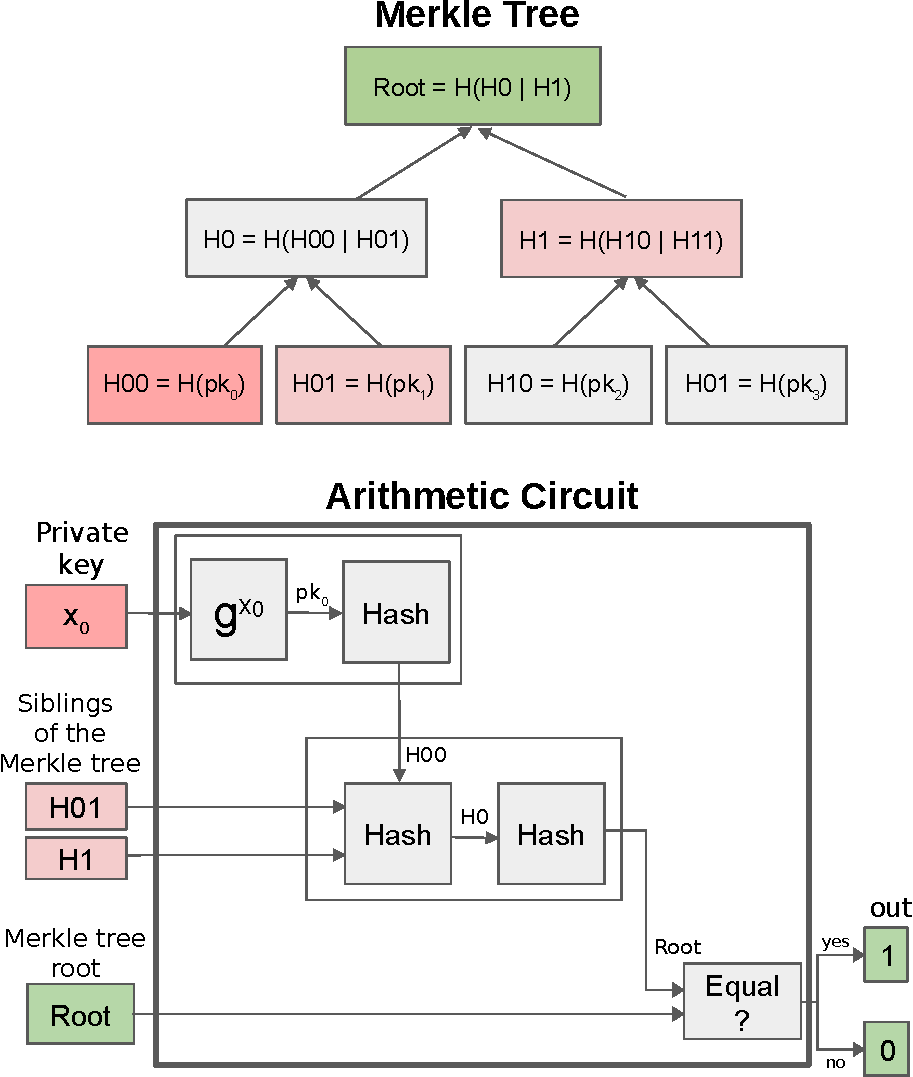
\includegraphics[width=1\columnwidth]{figures/tree_and_circuit}
	\caption{Merkle tree and arithmetic circuit design for a DAO membership proof. \label{fig:tree_and_circuit}}
	%TODO: Add public key to the upper box
\end{figure}

To preserve user-privacy, the private key and the Merkle proof are 
private inputs, whereas the root and the output are public values. 
As a result, any DAO member can generate a zero-knowledge membership 
proof using this circuit while keeping her inputs private. 
Attacks are not possible even for someone who knows all the values of 
the Merkle tree
since to fake a proof the circuit requires knowledge of an authorized private key. 
Moreover, this means that the DAO does not need to provide individual Merkle proofs to 
each member as before but simply can make the whole tree public. 

Circuit from Figure \ref{fig:tree_and_circuit} 
can be implemented using \texttt{circom} which 
has a library with a collection of templates that can be combined to 
create larger circuits. 
In our example, the circuit would simply be a combination of
the template that computes a public key given a private key, the template 
that computes a predefined hash function and the template that compares two values. 
The possibility of creating circuits by joining and combining small pieces of circuits 
makes programming in \texttt{circom} language very accessible to high level
practitioners. \\

Once the circuit is created, it can be compiled to obtain a JSON file that
contains a circuit representation.
Then, this JSON file is used as input of \texttt{snarkjs}
to generate the zero-knowledge proof.
The output of \texttt{snarkjs} is another JSON file containing 
a set of values that prove that the circuit was computed correctly 
but without revealing anything about the private inputs used. 
In this example, the proof shows that the prover holds a private key associated to 
an authorized public key of the DAO. 
Moreover, to easily validate zero-knowledge proofs on chain,
\texttt{snarkjs}
can generate the Solidity code to create a verifier in Ethereum
(for further details of \texttt{snarkjs} see \cite{snarkjs}).

Finally, the last step would be that a DAO member sends a transaction 
to the smart contract including the zero-knowledge proof. 
In our previous non-ZKP model, it was necessary to check 
that the transaction signature was produced using a public 
key that belongs to the tree.
In this privacy-enabled model, the proof already shows that the sender knows one of the authorized private keys.
But, anyway, a transaction has to be sent to the DAO smart contract 
including the proof.
If the member uses her private key to sign this transaction, 
she would loose her anonymity.
To obfuscate the member's identity, a simple solution is to 
send the transaction from any another account or use a relayer.

\section{CONCLUSION}

The key aspect of privacy-enabled blockchain applications is that they 
allow performing transactions that honour certain logic dependant on 
private data using a public transparent ledger.
Currently, there is a need to make privacy-enabled applications
more accessible in blockchain networks with smart contract capabilities like Ethereum. 
In this paper, we contribute to this necessity by describing a use case of how to build a privacy-enabled blockchain application and presenting our software tools to
make this process easier and clearer for high level practitioners.

\bibliographystyle{ieeetr}
\bibliography{bib/lit.bib}

\begin{IEEEbiography}{Marta Bell\'es-Mu\~noz}{\,}is currently a PhD student doing research  
in security and efficiency of arithmetic circuits for zero-knowledge 
protocols at Universitat Pompeu Fabra in collaboration with iden3. 
She receieved her B.S. degree in Mathematics at Universitat Autònoma de Barcelona 
and continued her Master studies at Aarhus Univeristy, where she focused on the 
study of elliptic curves and isogeny based cryptography. 
She has been part of the team developing Baby Jubjub elliptic curve for Ethereum and 
has been involved in the standardisation process for generating new elliptic curves 
inside zk-SNARK circuits. Contact her at marta@iden3.com.
\end{IEEEbiography}

\begin{IEEEbiography}{Jordi Baylina}{\,}is one of the most 
outstanding members of Ethereum community and author of several 
Ethereum Improvement Proposals 
(EIP165, EIP672, EIP777, EIP820, E1820, EIP2046)  
and relevant smart contracts. 
He is also part of the White Hat Group, with whom he participated in the DAOs and 
Parity Multisig hack rescues, recovering more than 300 million euros. 
He received his B.S. degree in Telecommunications Engineering from Universitat
Politècnica de Catalunya and his current research interests are applied
cryptography, zero-knowledge proofs and distributed ledger technologies. 
He is the co-founder and technical lead of iden3 and the main contributor to  
\texttt{circom} and \texttt{snarkjs} software. Contact him at jordi@baylina.cat.	
\end{IEEEbiography}

\begin{IEEEbiography}{Vanesa Daza}{\,}is with Pompeu Fabra University as 
Associate Professor since 2012. 
She holds a B.S. degree from Universitat de Barcelona and a Ph.D. in 
Mathematics from Universitat Politècnica de Catalunya.
She is the co-author of more than 40 papers, including international
journals and top conferences of cryptography and cybersecurity, and
co-inventor of three international patents. 
She is an Associate Editor of IEEE Transactions 
on Dependable and Secure Computing and IEEE Transactions on Information Forensics 
and Security. 
Her main research interests are distributed cryptographic 
techniques to improve security and privacy of blockchain technologies. 
Contact her at vanesa.daza@upf.edu.
\end{IEEEbiography}

\begin{IEEEbiography}{Jos\'e L. Mu\~noz}{\,}is a researcher of the Information Security Group (ISG) 
and an associate professor of the Department of Network Engineering of the Universitat Politècnica 
of Catalunya (UPC).
He holds a M.S. in Telecommunications Engineering (1999) and a PhD in Security Engineering (2003).
He has worked in applied cryptography, network security and game theory models applied to networks and simulators.
His research focus has now tuned to distributed ledgers technologies and he is the director of the master program 
in Blockchain technologies at UPC School. Contact him at jose.luis.munoz@upc.edu.
\end{IEEEbiography}

\end{document}